
\documentclass[
   ngerman          % neue deutsche Rechtschreibung
  ,a4paper          % Papiergrösse
% ,twoside          % Zweiseitiger Druck (rechts/links)
% ,10pt             % Schriftgrösse
%,11pt
  ,12pt
  ,pdftex
  ,disable         % Todo-Markierungen auschalten
]{report}

% Bitte die Codierung Ihrer Dateien auswählen:
% \usepackage[latin1]{inputenc}    % Für UNIX mit ISO-LATIN-codierten Dateien
% \usepackage[applemac]{inputenc}  % Für Apple Mac
% \usepackage[ansinew]{inputenc}   % Für Microsoft Windows
\usepackage[utf8]{inputenc}        % UTF-8 codierte Dateien
                                   % Dieses Dokument ist unter Unix erstellt, daher
                                   % wird diese Input-Codierung benutzt.

\usepackage{bericht}
\usepackage{graphicx}
\usepackage{listings}
\lstset{numbers=left, numberstyle=\tiny, numbersep=5pt}
\lstset{language=[Sharp]C}
%\usepackage{hyperref}
\graphicspath{{images/}}
\usepackage[onehalfspacing]{setspace}
\usepackage{float}
\renewcommand\topfraction{.9}
\renewcommand\textfraction{0.35}
\renewcommand\floatpagefraction{0.8}

%% ACHTUNG, wenn man eine eigene Formatdatei (bericht.fmt) benutzt, werden Änderungen an bericht.sty
%% erst wirksam, wenn die Format-Datei neu erzeugt wurde!!!
%% Genauer alle Änderungen, die textuell vor der nächsten Zeile ".... endofdump...." stehen
%% werden erst wirksam, wenn die Formatdatei neu erzeugt wurde
\csname endofdump\endcsname

%%%%%%%%%%%%%%%%%%%%%%%%%%%%%%%%%%%%%%%%%%%%%%%%%%%%%%%%%%%%%%%%%%%%%%%%%%%%%%%
%% Angaben zur Arbeit
%%%%%%%%%%%%%%%%%%%%%%%%%%%%%%%%%%%%%%%%%%%%%%%%%%%%%%%%%%%%%%%%%%%%%%%%%%%%%%%

\newcommand{\Autor}{Jonas Kölblin}
\newcommand{\MatrikelNummer}{7150881}
\newcommand{\Kursbezeichnung}{TINF20B5}

\newcommand{\FirmenName}{SICK AG}
\newcommand{\FirmenStadt}{Waldkirch}

%\newcommand{\FirmenLogo}{\fbox{\includegraphics[width=4cm]{logo.pdf}}}
\newcommand{\DHLogo}{\fbox{
\includegraphics[width=4cm]{dhbw-logo.pdf}}}
% Falls es kein Firmenlogo gibt:
%  \newcommand{\FirmenLogoDeckblatt}{}

%\newcommand{\BetreuerFirma}{}
 \newcommand{\BetreuerDHBW}{Ralf Brune}

%%%%%%%%%%%%%%%%%%%%%%%%%%%%%%%%%%%%%%%%%%%%%%%%%%%%%%%%%%%%%%%%%%%%%%%%%%%%%%%%%%%%%

% Wird auf dem Deckblatt und in der Erklärung benutzt:
%\newcommand{\Was}{Projekt-/Studien-/Bachleorarbeit}
%\newcommand{\Was}{Projektarbeit}
\newcommand{\Was}{Studienarbeit}
%\newcommand{\Was}{Bachleorarbeit}

%%%%%%%%%%%%%%%%%%%%%%%%%%%%%%%%%%%%%%%%%%%%%%%%%%%%%%%%%%%%%%%%%%%%%%%%%%%%%%%%%%%%%

\newcommand{\Titel}{Automotive Security}
\newcommand{\AbgabeDatum}{22. Mai 2023} 

\newcommand{\Dauer}{24 Wochen}

% \newcommand{\Abschluss}{Bachelor of Engineering}
\newcommand{\Abschluss}{Bachelor of Science}

%\newcommand{\Studiengang}{Informatik / Informationstechnik}
\newcommand{\Studiengang}{Informatik / Angewandte Informatik}
\newcommand*{\quelle}{%
\footnotesize Quelle:
}
\hypersetup{%%
  pdfauthor={\Autor},
  pdftitle={\Titel},
  pdfsubject={\Was}
}

%%%%%%%%%%%%%%%%%%%%%%%%%%%%%%%%%%%%%%%%%%%%%%%%%%%%%%%%%%%%%%%%%%%%%%%%%%%%%%%

% Wenn \includeonly{..} benutzt wird, werden nur diese Kaptitel ausgegeben.
\includeonly{
  abk
% ,changelog
 ,abstract
 ,Einführung
 ,Grundlagen
 ,Ausarbeitung
 ,Fazit
}

%%%%%%%%%%%%%%%%%%%%%%%%%%%%%%%%%%%%%%%%%%%%%%%%%%%%%%%%%%%%%%%%%%%%%%%%%%%%%%%

% Benutzt man das "biblatex"-Paket, dann muß das hier stehen:
% siehe auch die mit BIBLATEX markierten Zeilen in bericht.sty
\bibliography{bericht}

\begin{document}

%%%%%%%%%%%%%%%%%%%%%%%%%%%%%%%%%%%%%%%%%%%%%%%%%%%%%%%%%%%%%%%%%%%%%%%%%%%%%%%

\begin{titlepage}
\begin{center}
\vspace*{-2cm}
%\includegraphics[width=4cm]{logo.pdf}
\hfill
\includegraphics[width=4cm]{dhbw-logo}\\[2cm]
{\Huge \Titel}\\[1cm]
{\Huge\scshape \Was}\\[1cm]
{\large für die Prüfung zum}\\[0.5cm]
{\Large \Abschluss}\\[0.5cm]
{\large des Studienganges \Studiengang}\\[0.5cm]
{\large an der}\\[0.5cm]
{\large Dualen Hochschule Baden-Württemberg Karlsruhe}\\[0.5cm]
{\large von}\\[0.5cm]
{\large\bfseries \Autor}\\[1cm]
{\large Abgabedatum \AbgabeDatum}
\vfill
\end{center}
\begin{tabular}{l@{\hspace{2cm}}l}
Bearbeitungszeitraum	         & \Dauer 			\\
Matrikelnummer	                 & \MatrikelNummer		\\
Kurs			         & \Kursbezeichnung		\\
Ausbildungsfirma	         & \FirmenName			\\
			         & \FirmenStadt			\\
%Betreuer der Ausbildungsfirma	 & \BetreuerFirma		\\
Gutachter der Studienakademie	 & \BetreuerDHBW		\\
\end{tabular}
\end{titlepage}

%%%%%%%%%%%%%%%%%%%%%%%%%%%%%%%%%%%%%%%%%%%%%%%%%%%%%%%%%%%%%%%%%%%%%%%%%%%%%%%

%%%%%%%%%%%%%%%%%%%%%%%%%%%%%%%%%%%%%%%%%%%%%%%%%%%%%%%%%%%%%%%%%%%%%%%%%%%%%%%
%% Descr:       Vorlage für Berichte der DHBW-Karlsruhe, Erklärung
%% Author:      Prof. Dr. Jürgen Vollmer, vollmer@dhbw-karlsruhe.de
%% $Id: erklaerung.tex,v 1.11 2020/03/13 14:24:42 vollmer Exp $
%% -*- coding: utf-8 -*-
%%%%%%%%%%%%%%%%%%%%%%%%%%%%%%%%%%%%%%%%%%%%%%%%%%%%%%%%%%%%%%%%%%%%%%%%%%%%%%%

% In Bachelorarbeiten muss eine schriftliche Erklärung abgegeben werden.
% Hierin bestätigen die Studierenden, dass die Bachelorarbeit, etc.
% selbständig verfasst und sämtliche Quellen und Hilfsmittel angegeben sind. Diese Erklärung
% bildet das zweite Blatt der Arbeit. Der Text dieser Erklärung muss auf einer separaten Seite
% wie unten angegeben lauten.

\newpage
\thispagestyle{empty}
\begin{framed}
\begin{center}
\Large\bfseries Erklärung
\end{center}
\medskip
\noindent
% siehe §5(3) der \enquote{Studien- und Prüfungsordnung DHBW Technik} vom 29.\,9.\,2017 und Anhang 1.1.13
Ich versichere hiermit, dass ich meine \Was{} mit dem Thema:
\enquote{\Titel}
selbstständig verfasst und keine anderen als die angegebenen Quellen und Hilfsmittel benutzt habe. Ich versichere zudem, dass die eingereichte elektronische Fassung mit der gedruckten Fassung übereinstimmt. \\
\vspace{3cm} \\
\noindent
\underline{\hspace{4cm}}\hfill\underline{\hspace{6cm}}\\
Ort~~~~~Datum\hfill Unterschrift\hspace{4cm}
\end{framed}

\vfill

%\begin{framed}
%\begin{center}
%\Large\bfseries Sperrvermerk
%\end{center}
%\medskip
%\noindent
%Der Inhalt dieser Arbeit darf weder als Ganzes noch in Auszügen Personen
%außerhalb des Prüfungsprozesses und des Evaluationsverfahrens zugänglich gemacht
%werden, sofern keine anderslautende Genehmigung vom Dualen Partner vorliegt.
%\end{framed}

%%%%%%%%%%%%%%%%%%%%%%%%%%%%%%%%%%%%%%%%%%%%%%%%%%%%%%%%%%%%%%%%%%%%%%%%%%%%%%%
\endinput
%%%%%%%%%%%%%%%%%%%%%%%%%%%%%%%%%%%%%%%%%%%%%%%%%%%%%%%%%%%%%%%%%%%%%%%%%%%%%%%


%%%%%%%%%%%%%%%%%%%%%%%%%%%%%%%%%%%%%%%%%%%%%%%%%%%%%%%%%%%%%%%%%%%%%%%%%%%%%%%

%\begin{abstract}
%Dieses \LaTeX-Dokument kann als Vorlage für einen Praxis- oder Projektbericht, eine Studien- oder
%Bachelorarbeit dienen.

%Zusammengestellt von Prof.\,Dr.\,Jürgen Vollmer \email{juergen.vollmer@dhbw-karlsruhe.de}\\
%\url{https://www.karlsruhe.dhbw.de}. Die jeweils aktuellste Version dieses \LaTeX-Paketes ist immer
%auf der \emph{FAQ-Seite} des Studiengangs Informatik zu finden:
%\url{https://www.karlsruhe.dhbw.de/inf/studienverlauf-organisatorisches.html} $\to$ \emph{Formulare und Vorlagen}.%

%\centering Stand \verb+$Date: 2020/03/13 15:07:45 $+
%\end{abstract}

\newpage
\pagenumbering{Roman}
\chapter*{Abstract}
In dieser Arbeit wird ein Überblick über das Gebiet der Automotive Cyber Security geschaffen, mit dem Ziel, aufzuzeigen, wie sicher die heutigen Automobile sind und wo Automobilhersteller ansetzen können, um ihre Fahrzeuge sicherer zu machen.\\
Hierzu werden die in Automotive Netzwerken verwendeten Standards und die wichtigsten Grundlagen der Cyber Security erläutert. Anschließend erfolgt eine Untersuchung und Risikoabschätzung bekannter Angriffsflächen von Automobilen. Danach werden Schutzmaßnahmen und Ansätze vorgestellt, wie mit Hilfe des Defense-In-Depth-Prinzips die Sicherheit der Fahrzeuge gegen Angriffe erhöht werden kann. Zudem wird am Ende noch ein kurzer Blick auf die besonderen Herausforderungen der Automotive Security geworfen.\\
Am Ende werden die erarbeiteten Ergebnisse nochmals betrachtet, ein Fazit gezogen und weitere Handlungsempfehlungen für die Hersteller vorgeschlagen.
\tableofcontents           % Inhaltsverzeichnis hier ausgeben
\listoffigures             % Liste der Abbildungen
%\listoftables              % Liste der Tabellen
%\lstlistoflistings         % Liste der Listings
%\listofequations           % Liste der Formeln

% Jetzt kommt der "eigentliche" Text
%
%%%%%%%%%%%%%%%%%%%%%%%%%%%%%%%%%%%%%%%%%%%%%%%%%%%%%%%%%%%%%%%%%%%%%%%%%%%%%%
%% Descr:       Vorlage für Berichte der DHBW-Karlsruhe, Datei mit Abkürzungen
%% Author:      Prof. Dr. Jürgen Vollmer, vollmer@dhbw-karlsruhe.de
%% $Id: abk.tex,v 1.4 2017/10/06 14:02:03 vollmer Exp $
%% -*- coding: utf-8 -*-
%%%%%%%%%%%%%%%%%%%%%%%%%%%%%%%%%%%%%%%%%%%%%%%%%%%%%%%%%%%%%%%%%%%%%%%%%%%%%%%

\chapter*{Abkürzungsverzeichnis}                   % chapter*{..} -->   keine Nummer, kein "Kapitel"
						         % Nicht ins Inhaltsverzeichnis
% \addcontentsline{toc}{chapter}{Akürzungsverzeichnis}   % Damit das doch ins Inhaltsverzeichnis kommt

% Hier werden die Abkürzungen definiert
\begin{acronym}[DHBW]
  % \acro{Name}{Darstellung der Abkürzung}{Langform der Abkürzung}
  %SICK
 \acro{Abk}[Abk.]{Abkürzung}
 \acro{GBC}[GBC]{Global Business Center}
 \acro{CD}[CD]{Corporate Department}
 \newacroplural{CD}[CD]{Corporate Departments}
 \acro{DMT}[DMT]{Digital Manufacturing Team}
 \acro{ISN}[ISN]{Intelligent Supply Network}
 \acro{BU}[BU]{Business Unit}
 
 %Automotive
 \acro{ECU}[ECU]{Electronic Control Unit}
 \newacroplural{ECU}[ECUs]{Electronic Control Units}
 \acro{CAN}[CAN]{Controller Area Network}
 \acro{DLC}[DLC]{Data Link Connector}
 \acro{LIN}[LIN]{Local Interconnect Network}
 
 %Testing
 \acro{ISTQB}[ISTQB]{International Software Testing Qualification Board}
 \acro{SUT}[SUT]{System under Test}
 
 %Allgemein
 \acro{HTML}[HTML]{Hypertext Markup Language}
 \acro{UI}[UI]{User Interface}
 \acro{API}[API]{Application Programming Interface}
 \acro{MVC}[MVC]{Model View Controller}

 \acro{IDE}[IDE]{Integrated Development Environment}
 % Folgendes benutzen, wenn der Plural einer Abk. benöigt wird
 % \newacroplural{Name}{Darstellung der Abkürzung}{Langform der Abkürzung}
 \newacroplural{Abk}[Abk-en]{Abkürzungen}

 \acro{H2O}[\ensuremath{H_2O}]{Di-Hydrogen-Monoxid}

 % Wenn neicht benutzt, erscheint diese Abk. nicht in der Liste
 \acro{NUA}{Not Used Acronym}
\end{acronym}
              % Abkürzungsverzeichnis
\newpage
\pagenumbering{arabic}
\include{Einführung}
\chapter{Grundlagen}
In diesem Kapitel sollen die für das weitere Verständnis notwendigen theoretischen Grundlagen erläutert werden. Dazu gehört zunächst der Aufbau des Netzwerks in einem Fahrzeug. Des Weiteren werden relevante Grundlagen der Cyber Security erklärt.

\section{Automotive Networking}
Im Inneren von Autos befinden sich heutzutage eine Vielzahl elektronischer Systeme, von denen jedes mit benachbarten Komponenten kommunizieren kann. Die einzelnen elektronischen Systeme werden als \acp{ECU} bezeichnet. Moderne Autos enthalten in der Regel über 50 verschiedene \acsp{ECU} \cite[vgl.][6]{Miller.2013}. Da diese Kontrolleinheiten zum Teil lebensentscheidende Aufgaben übernehmen, muss die Kommunikation zwischen den Einheiten möglichst in Echtzeit erfolgen. \\

\begin{figure}[H]
\centering
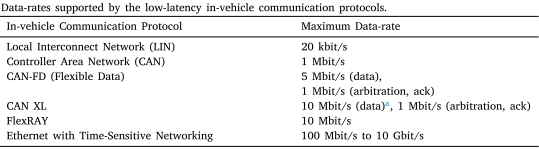
\includegraphics[width=\textwidth]{communication-protocols}
\label{fig:communication-protocols}
\caption{Verschiedene Kommunikationsprotokolle in Automobil-Netzwerken}
\quelle{\cite[2]{MohammadAshjaei.2021}}
\end{figure}

Für die Venetzung der \acsp{ECU} kommen verschiedene Technologien zum Einsatz (siehe Abbildung \ref{fig:communication-protocols}). Diese werden im Folgenden genauer erläutert. Die relevanteste davon ist im Automotive-Bereich der sogenannte \acs{CAN}-Standard.

\subsection{Controller Area Network}
Die elektronischen Kontrolleinheiten eines Autos sind typischerweise über einen oder mehrere Busse, die auf dem \ac{CAN}-Standard basieren, miteinander verbunden. Hierbei kommunizieren die \acsp{ECU} über \acs{CAN}-Pakete. Diese werden an alle Komponenten gesendet, welche dann jeweils basierend auf dem Inhalt entscheiden, ob das Paket für sie bestimmt ist oder nicht. Eine Identifikation der Quelle oder Authentisierung gibt es in diesem Standard nicht. \cite[vgl.][7]{Miller.2013} \\
In Abbildung \ref{fig:canbus-ford2010} ist das \acs{CAN}-Netzwerk eines 2010 Ford Escape dargestellt. Das abgebildete Netzwerk verfügt über zwei Busse, einen medium speed (MS) und einen high speed (HS) \acs{CAN}-Bus. Beide Busse enden hier im \ac{DLC} (siehe Kapitel \ref{OBD-II}).
In Automotive Netzwerken lassen sich zwei Arten von \acs{CAN}-Paketen finden: normale \acs{CAN}-Pakete und diagnostische \acs{CAN}-Pakete. 

\begin{figure}[h]
\centering
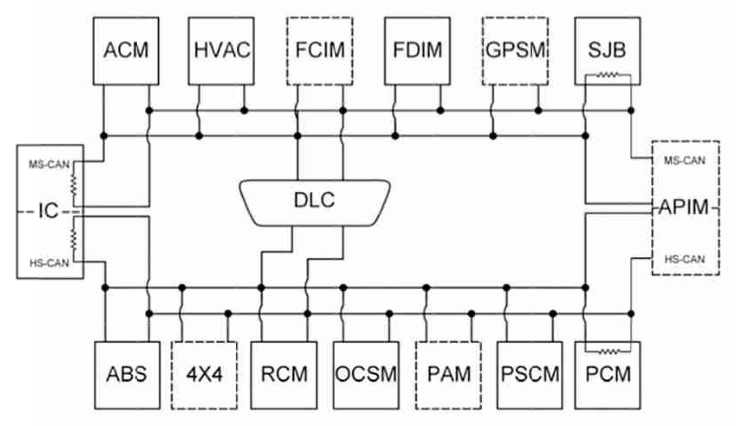
\includegraphics[width=\textwidth]{Miller_canbus-ford2010}
\label{fig:canbus-ford2010}
\caption{Beispiel des \acs{CAN}-Netzwerks eines 2010 Ford Escape}
\quelle{\cite[19]{Miller.2013}}
\end{figure}

\subsubsection{Normale \acs{CAN}-Pakete}
Normale Pakete werden von \acsp{ECU} gesendet und können entweder Informationen oder Befehle enthalten. Typischerweise werden sie alle Millisekunden gesendet. Auf Anwendungsebene enthalten die \acs{CAN}-Pakete einen Identifier, die zu übertragenden Daten und manchmal noch eine Prüfsumme, um sicherzustellen, dass das Paket korrekt übertragen wurde. Der Identifier gibt sowohl an, für welche \acsp{ECU} das Paket bestimmt ist, als auch, welche Priorität das Paket hat. \cite[vgl.][9]{Miller.2013}

\subsubsection{Diagnostische \acs{CAN}-Pakete}
Diagnostische Pakete tauchen während des normalen Betriebs des Autos im Normalfall nicht auf. Sie werden von Diagnose-Werkzeugen gesendet, die beispielsweise von Mechanikern genutzt werden um mit den \acsp{ECU} im Auto zu kommunizieren. So können Mängel und Fehlfunktionen entdeckt oder andere Informationen gewonnen werden. Das Format von diagnostischen \acs{CAN}-Paketen ähnelt dem von normalen Paketen, erfolgt jedoch meist nach strengeren Konventionen. Standards hierfür sind zum Beispiel ISO-TP, ISO 14229 und ISO 14230. \cite[vgl.][10]{Miller.2013}



\subsection{Schnittstellen}
\subsubsection{OBD-II Port} \label{OBD-II}

\section{Cyber Security}
\chapter{Angriffsflächen}


\chapter{Schutzmaßnahmen}
\chapter{Fazit}
\section{Schlussfolgerung}

\section{Ausblick}


% Ab hier beginnt der Anhang
\appendix
%\addcontentsline{toc}{chapter}{Anhang}

%\addcontentsline{toc}{chapter}{Index}
\printindex

\addcontentsline{toc}{chapter}{Literaturverzeichnis}

% Haben Sie das "biblatex"-Paket nicht installiert, benutzen Sie folgendes:
% Ohne das "biblatex"-Paket (s. bericht.sty) produziert folgendes
% "deutsche" Zitate in Literaturverzeichnissen gemaß der Norm DIN 1505,
% Teil 2 vom Jan. 1984.
% Die Zitatmarken werden alphabetisch nach Verfassern
% sortiert und sind durch abgekürzte Verfasserbuchstaben plus
% Erscheinungsjahr in eckigen Klammern gekennzeichnet.

% \bibliographystyle{alphadin}
% \bibliography{bericht}

%%%%%%%%%%%%%%%%%%%%%%%%%%%%%%%%%%%%%%%5
% BIBLATEX
% Benutzt man das "biblatex"-Paket, muß man folgendes schreiben:
\def\refname{bericht}
\printbibliography
%%%%%%%%%%%%%%%%%%%%%%%%%%%%%%%%%%%%%%%5


%\include{changelog}

%\newpage
%\addcontentsline{toc}{chapter}{Liste der ToDo's}
%\listoftodos[Liste der ToDo's]


\end{document}
